\documentclass{standalone}
\begin{document}
\subsection{Gamma Correction}

Medical digital images can suffer from poor contrast\cite{gammacorr1}. 
In order to prevent information loss and to appreciate all the details of the image, it is necessary to enhance the contrast of such images. 
There are numerous existing techniques that can be performed for this purpose.
In this work, I performed gamma correction.
\\
It consists of a non-linear operation, defined in the simplest cases, by the following power-law expression:

\begin{equation}
    I_{out} = C I_{in}^{\gamma}
\end{equation}

where the output $I_{out}$ is obtained multiplying by a constant $C$ the input value $I_{in}$ raised to the power $\gamma$.
A value of $\gamma < 1$ is sometimes called an encoding gamma; conversely a gamma value $\gamma > 1$ is called a decoding gamma.
In practice, powers of $\gamma$ larger than 1 make the shadows darker, while powers smaller than 1 make dark regions lighter.
\\
In particular, for this work, the gamma correction was performed by the following expression: 
\begin{equation}
    I_{out} =  (\frac{I_{in} - I_{min}}{I_{max} - I_{min}})^{\gamma}
\end{equation}
where $I_{min}, \: I_{max}$ are respectively the minimum and the maximum image value.

\begin{figure}[!htp]

    \centering
    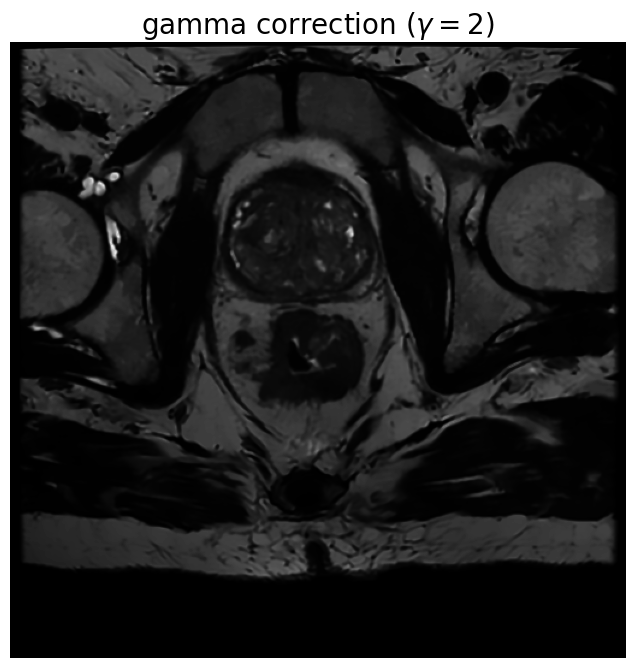
\includegraphics[width=.33\textwidth]{../images/gamma_2.png}\hfill
    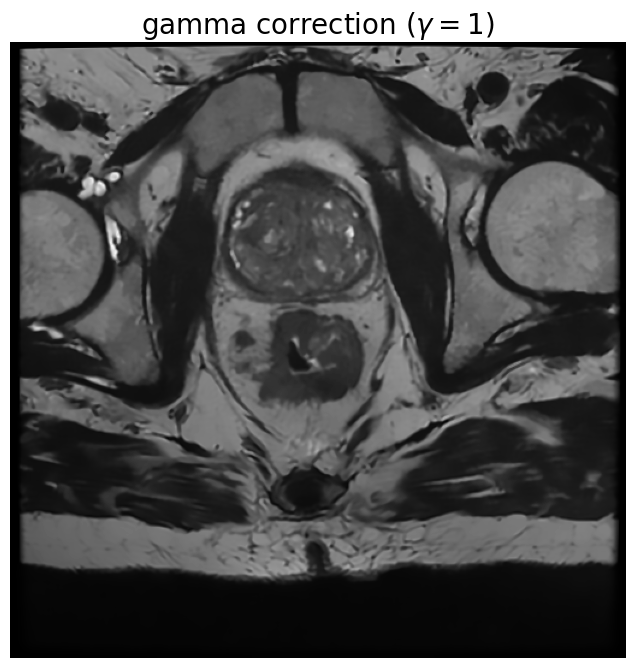
\includegraphics[width=.33\textwidth]{../images/gamma_1.png}\hfill
    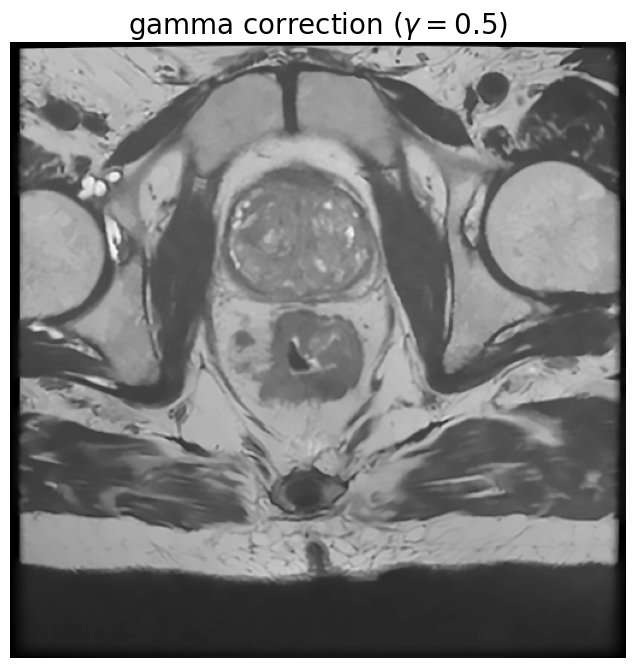
\includegraphics[width=.33\textwidth]{../images/gamma_1.5.png}
    
\caption{Example of gamma correction, applied to a MR image, varying $\gamma$.
As you can see, a value of $\gamma$ larger than 1 enhances darker regions while a value smaller than 1 makes dark regions lighter; a value of $\gamma$ equal to 1 corresponds to the original image.
Images from IRCCS Sant’Orsola-Malpighi Policlinic Dataset.}
    
\end{figure}

\end{document}